\chapter{Técnicas y métodos de detección}\label{chap:tecnicas}
Existe una gran variedad de técnicas y métodos de detección de anomalías, si bien cada uno
de ellos tiene sus propias ventajas y desventajas. Es importante tener en cuenta que la
efectividad de cada uno de ellos depende en gran medida del tipo de datos que se esté
tratando, además del propio método en sí.

Por ejemplo, algunos algoritmos de detección están diseñados para detectar anomalías \textit{locales},
mientras que otros están diseñados para detectar anomalías \textit{globales}. Casi todos los algoritmos
requieren que se establezan parámetros de entrada poco intuitivos o incluso desconocidos previo
al propio análisis de los datos, como el número de vecinos más cercanos o umbrales de distancia.

\section{Categorías y etiquetas de clase}
Existen tres grandes categorías de tećnicas de detección de anomalías, dependiendo de la información
sobre los datos de la que se disponga:

\begin{itemize}[topsep=0pt]
	\item \textbf{Detección supervisada:} estas técnicas requieren un conjunto de datos etiquetado
		que contenga tanto datos normales como datos anómalos. El objetivo de estas técnicas es
		crear un \textit{clasificador} que sea capaz de distinguir entre ambos tipos de datos. \\
		Este enfoque no se utiliza frecuentemente, ya que en la práctica es muy difícil obtener
		un conjunto de datos etiquetado por la naturaleza de los datos que se quieren analizar.
	\item \textbf{Detección no supervisada:} cuando no se dispone de datos etiquetados, se puede
		tratar de asociar una \textit{\textbf{puntuación}} a cada objeto en función de la probabilidad que
		se estime de que dicho objeto sea una anomalía. En este caso, no se puede distinguir entre
		diferentes tipos de anomalías, sino que se trata de detectar cualquier tipo de anomalía. \\
		Para que este enfoque funcione, debe existir una diferencia significativa entre los datos
		normales y los considerados \textit{anómalos}.
	\item \textbf{Detección semi-supervisada:} este conjunto de técnicas se puede utilizar cuando se
		cuentan con datos categorizados como \textit{normales} pero NO datos etiquetados como anómalos.
		En este caso, se utiliza un algoritmo para asignar un grado de anormalidad a cada objeto en
		funciónde la información que se tenga de los datos normales. Normalmente, se entrena un
		modelo con los datos normales y se decide si un objeto es anómalo o no si se ajusta al modelo.
\end{itemize}

\section{Enfoques}
Para tratar de resolver el problema de la detección, se han desarrollado una gran variedad de
técnicas y métodos. Los siguientes enfoques son los más comunes:
\begin{itemize}[topsep=0pt]
	\item \textbf{Técnicas basadas en modelos (\textit{estadísticas}):} en este caso, los anomalías serán
		aquellos objetos que no se ajusten bien al modelo que se haya generado previamente. Por ejemplo,
		si se están trabajando en un problema de regresión, las anomalías serán aquellas que tengan un
		gran error de predicción. Dentro de la detección estadística, se distinguen varios tipos de detección:
		(\textbf{probabilística}, \textbf{de outliers} y \textbf{de \textit{novelties}}). Normalmente, se
		trabaja asumiendo que los datos siguen una distribución normal, lo que permite utilizar la media y la
		desviación en problemas univarpiantes o la distancia de \emph{Mahalanobis}~\cite{mahalanobis2018generalized}
		en problemas multivariantes.

		\begin{minipage}{\linewidth}
			\centering
			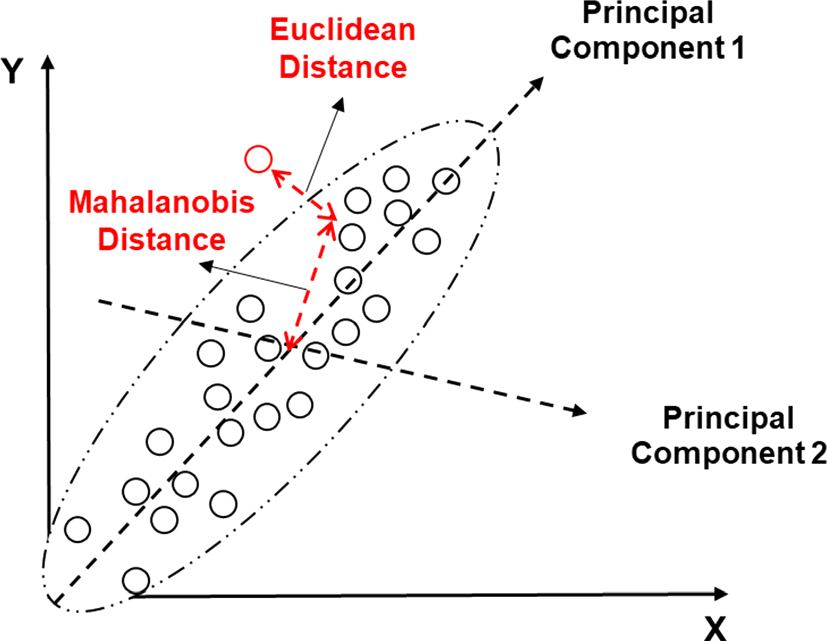
\includegraphics[width=\textwidth]{mahalanobis.png}
			\captionof{figure}{Distancia de Mahalanobis ($T^2$)
				y Euclídea ($Q$)~\cite{lee2020monitoring}}\label{fig:fig2}
		\end{minipage}
	\item \textbf{Técnicas basdadas en proximidad:} estas técnicas explotan una métrica de
		similaridad entre objetos para medir la \textit{distancia} entre ellos. Los objetos que
		se encuentren a una distancia mayor que un umbral establecido se considerarán anomalías.
		En caso de que se pueda representar los datos en un espacio bidimensional, se pueden
		detectar las anomalías a simple vista.

		\begin{minipage}{\linewidth}
			\centering
			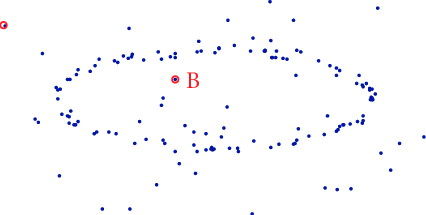
\includegraphics[width=\textwidth]{distance.png}
			\captionof{figure}{Dos tipos distintos de anomalías en la representación de un modelo
				de detección basado en proximidad~\cite{yu2010two}}\label{fig:fig4}
		\end{minipage}
	\item \textbf{Técnicas basadas en densidad:} considerando la densidad como \emph{el número de
		objetos en una región del espacio de datos}, los objetos que se encuentren en regiones
		con una baja densidad se pueden llegar a considerar anómalos. Normalmente se compara la
		densidad de un objeto con la densidad media de los objetos que se encuentran a su alrededor
		(vecinos más cercanos).
	\item \textbf{Técnicas basadas en clusters:} estas técnicas se basan en la idea de que los
		objetos normales pertenecen a un cluster o grupo, mientras que los objetos anómalos no
		pertenecen a ninguno. Por lo tanto, se puede detectar una anomalía si un objeto no pertenece
		a ningún cluster o si pertenece a un cluster con un número muy pequeño de objetos.
		\vspace{1\baselineskip}

		\begin{minipage}{\linewidth}
			\centering
			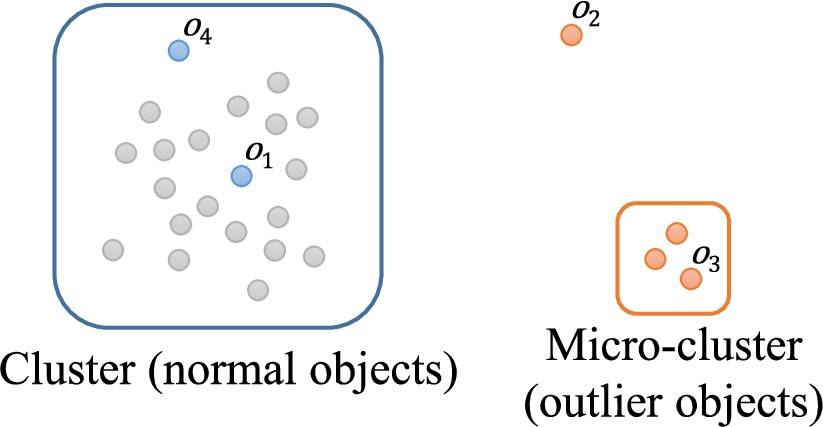
\includegraphics[width=\textwidth]{clusters.png}
			\captionof{figure}{Anomalías en un sistema de detección basado en
				clusters.~\cite{bae2020effective}}\label{fig:fig5}
		\end{minipage}
\end{itemize}

Dentro de los enfoques anteriores, se distinguen una gran variedad de técnicas más:
\begin{itemize}[noitemsep,topsep=0pt]
	\item Redes bayesianas
	\item Redes neuronales (replicantes, autocodificadores, de memoria a corto plazo)
	\item Modelos ocultos de Makarov (\textit{HMM})
	\item Técnicas de ensamblaje (usando \textit{feature bagging})
	\item Basadas en lógica difusa
	\item \textit{SVM} de una clase
\end{itemize}

Como anteriormente se ha mencionado, el rendimiento de cada una de estas técnicas depende
en gran medida del conjunto de datos y los parámetros escogidos, y no existe una ventaja
clara cuando se comparan entre sí utilizando muchos conjuntos de datos.~\cite{chandola2009anomaly}
